\documentclass{article}
\usepackage{graphicx}
\usepackage[margin=1.5cm]{geometry}
\usepackage{amsmath}

\begin{document}

\title{Monday Reading Assessment: Unit 4, Forces}
\author{Prof. Jordan C. Hanson}

\maketitle

\section{Chapter 4 - Forces}

\begin{enumerate}
\item A spring exerts a force $\vec{s} = -k \Delta\vec{x}$.  The displacement $\Delta\vec{x}$ is the amount the spring is stretched, and $k$ is a constant with units of Newtons per meter.  If a spring with $k = 50.0$ N/m is stretched by 10 cm, what is the force $\vec{s}$?
\begin{itemize}
\item A: -500 N
\item B: 500 N
\item C: -5 N
\item D: 5 N
\end{itemize}
\item 
\begin{figure}[ht]
\centering
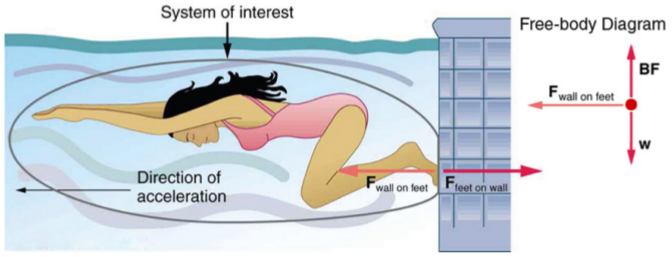
\includegraphics[width=0.4\textwidth,trim=0cm 0cm 4.75cm 2cm,clip=true]{wall.png}
\caption{\label{fig:wall} A woman pushes off of a wall underwater in a pool.}
\end{figure}
According to Fig. \ref{fig:wall}, a woman experiences a force by the wall on herself.  Her weight force $w$ is balanced by the buoyant force $BF$.  a) Draw a free body diagram for the system of interest.  b) If the wall exerts a force of 100 N, and her mass is 50 kg, what is her acceleration?
\item 
\begin{figure}[ht]
\centering
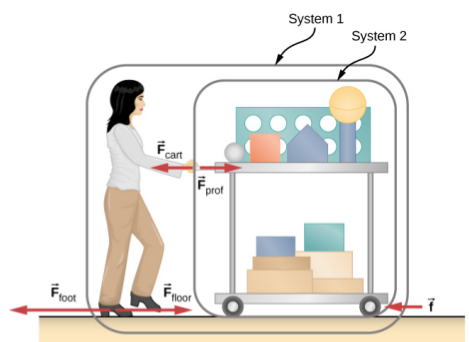
\includegraphics[width=0.4\textwidth]{cart.png}
\caption{\label{fig:cart} A woman pushes off of a wall underwater in a pool.}
\end{figure}
According to Fig. \ref{fig:cart}, a professor pushes an equipment cart.  The mass of the professor is 65.0 kg, the mass of the cart is 12.0 kg, and the mass of the equipment is 7.0 kg.  The professor exerts a backward force of 150.0 N on the floor.  There is a force of friction that exerts a force of 24.0 N to the left.  What is the acceleration of System 1?
\end{enumerate}

\end{document}
